\documentclass{beamer}
\mode<presentation>{\usetheme{Warsaw}}

\usepackage[citestyle=authortitle-icomp]{biblatex}
\usepackage[group-separator={,}]{siunitx}
\usepackage{tikz}
\usepackage{relsize}

\setbeamertemplate{caption}{\raggedright\insertcaption\par}
\setbeamerfont{caption}{size=\scriptsize}

\newcommand{\mathA}{\mathcal{A}}
\newcommand{\mathB}{\mathcal{B}}
\newcommand{\mathC}{\mathcal{C}}
\newcommand{\mathG}{\mathcal{G}}
\newcommand{\mathP}{\mathcal{P}}

\title[Bayesian Income Inference \hspace{3em} IEEE/ACM ASONAM 2016]{A Bayesian Approach to Income Inference \\ in a Communication Network}

\author[Fixman et.\ al]{%
	Martin~Fixman\inst{1}\inst{2}\and
	Jorge~Brea\inst{1}\and
	Ariel~Berenstein\inst{1}\and
	Carlos~Sarraute\inst{1}\and
	Martin~Minnoni\inst{1}\and
	Matias~Travizano\inst{1}
}

\institute{%
	\inst{1}Grandata Labs, Bartolome Cruz 1818, Vicente Lopez, Argentina \\
	\inst{2}Universidad de Buenos Aires, Argentina \bigbreak{}
	\{mfixman,ariel,jorge,martin,mat,charles\}@grandata.com
}

\date{}

\addbibresource{../bibliography/sna.bib}{}

\begin{document}

\begin{frame}
	\titlepage{}
\end{frame}

\section{Introduction}
\subsection{Introduction}

\begin{frame}{Introduction}
In recent years, we have witnessed an exponential growth in the capacity to gather, store and manipulate massive amounts of data across a broad spectrum of disciplines.

Mobile phone datasets provide a very rich view into the social interactions and the physical movements of large segments of a population.
\end{frame}

\subsection{Understanding the Social Graph}

\begin{frame}
The voice calls and text messages exchanged between people, together with the call locations (recorded through cell tower usages), allow us to construct a rich social graph which can give us interesting insights on the users' social fabric, detailing not only particular social relationships and traits, but also regular patterns of behavior both in space and time, such as their daily and weekly mobility patterns\footcite{gonzalez2008understanding}\footcite{ponieman2013human}\footcite{sarraute2015city}.
\begin{center}
\tikzstyle{att} = [circle, draw, fill=black!25, minimum size=10pt]
\tikzstyle{edge} = [draw, thick, >=latex]

\begin{tikzpicture}
	\node[att] (0) at (-2, 0) {};
	\node[att] (1) at (0, 0) {};
	\node[att] (2) at (0, -2) {};
	\node[att] (3) at (-2, -2) {};
	\node[att] (4) at (-1, -1) {};
	\node[att] (5) at (-3, -1) {};
	\path[edge, ->] (0) -- (1);
	\path[edge, ->] (1) -- (2);
	\path[edge, ->] (2) -- (3);
	\path[edge, <->] (3) -- (0);
	\path[edge, ->] (0) -- (4);
	\path[edge, <->] (4) -- (2);
	\path[edge, ->] (4) -- (3);
	\path[edge, <->] (5) -- (0);
	\path[edge, ->] (5) -- (3);

	\node[att] (a) at (1, 0) {};
	\node[att] (e) at (1, -1.5) {};
	\path[edge, <->] (1) -- (a);
	\path[edge, <-] (1) -- (e);
	\path[edge, ->] (2) edge [bend right = 30] (e);

	\path[edge, ->] (e) -- (a);
\end{tikzpicture}

\end{center}

\end{frame}

\begin{frame}
Economic factors are also believed to have a determining role in both the social network’s structure and dynamics. In particular, individuals have a tendency to establish links with others of a similar socioeconomic background, which results in social stratification\footcite{leo2015socioeconomic}.

\pause{}

In this work, we leverage the socioeconomic homophily present in the cellular phone network to generate inferences of socioeconomic status in the communication graph. To this aim we use two data sources:
\begin{enumerate}
	\item The Call Detail Records from the operator, which allows us to construct a social graph.
	\item Reported income from a subset of clients obtained from a large bank.
\end{enumerate}
\end{frame}

\section{Data Sources}
\subsection{Bank Data Source}

\begin{frame}{Bank Data Source}
For this study, we got access the account balances of over 10 million clients of a mexican bank for a period of 6 months, denoted \( \mathB \). We also have some demografic information of a subset \( \mathA \subseteq \mathB \), including the users' age.

\begin{figure}[h]
	\begin{center}
		{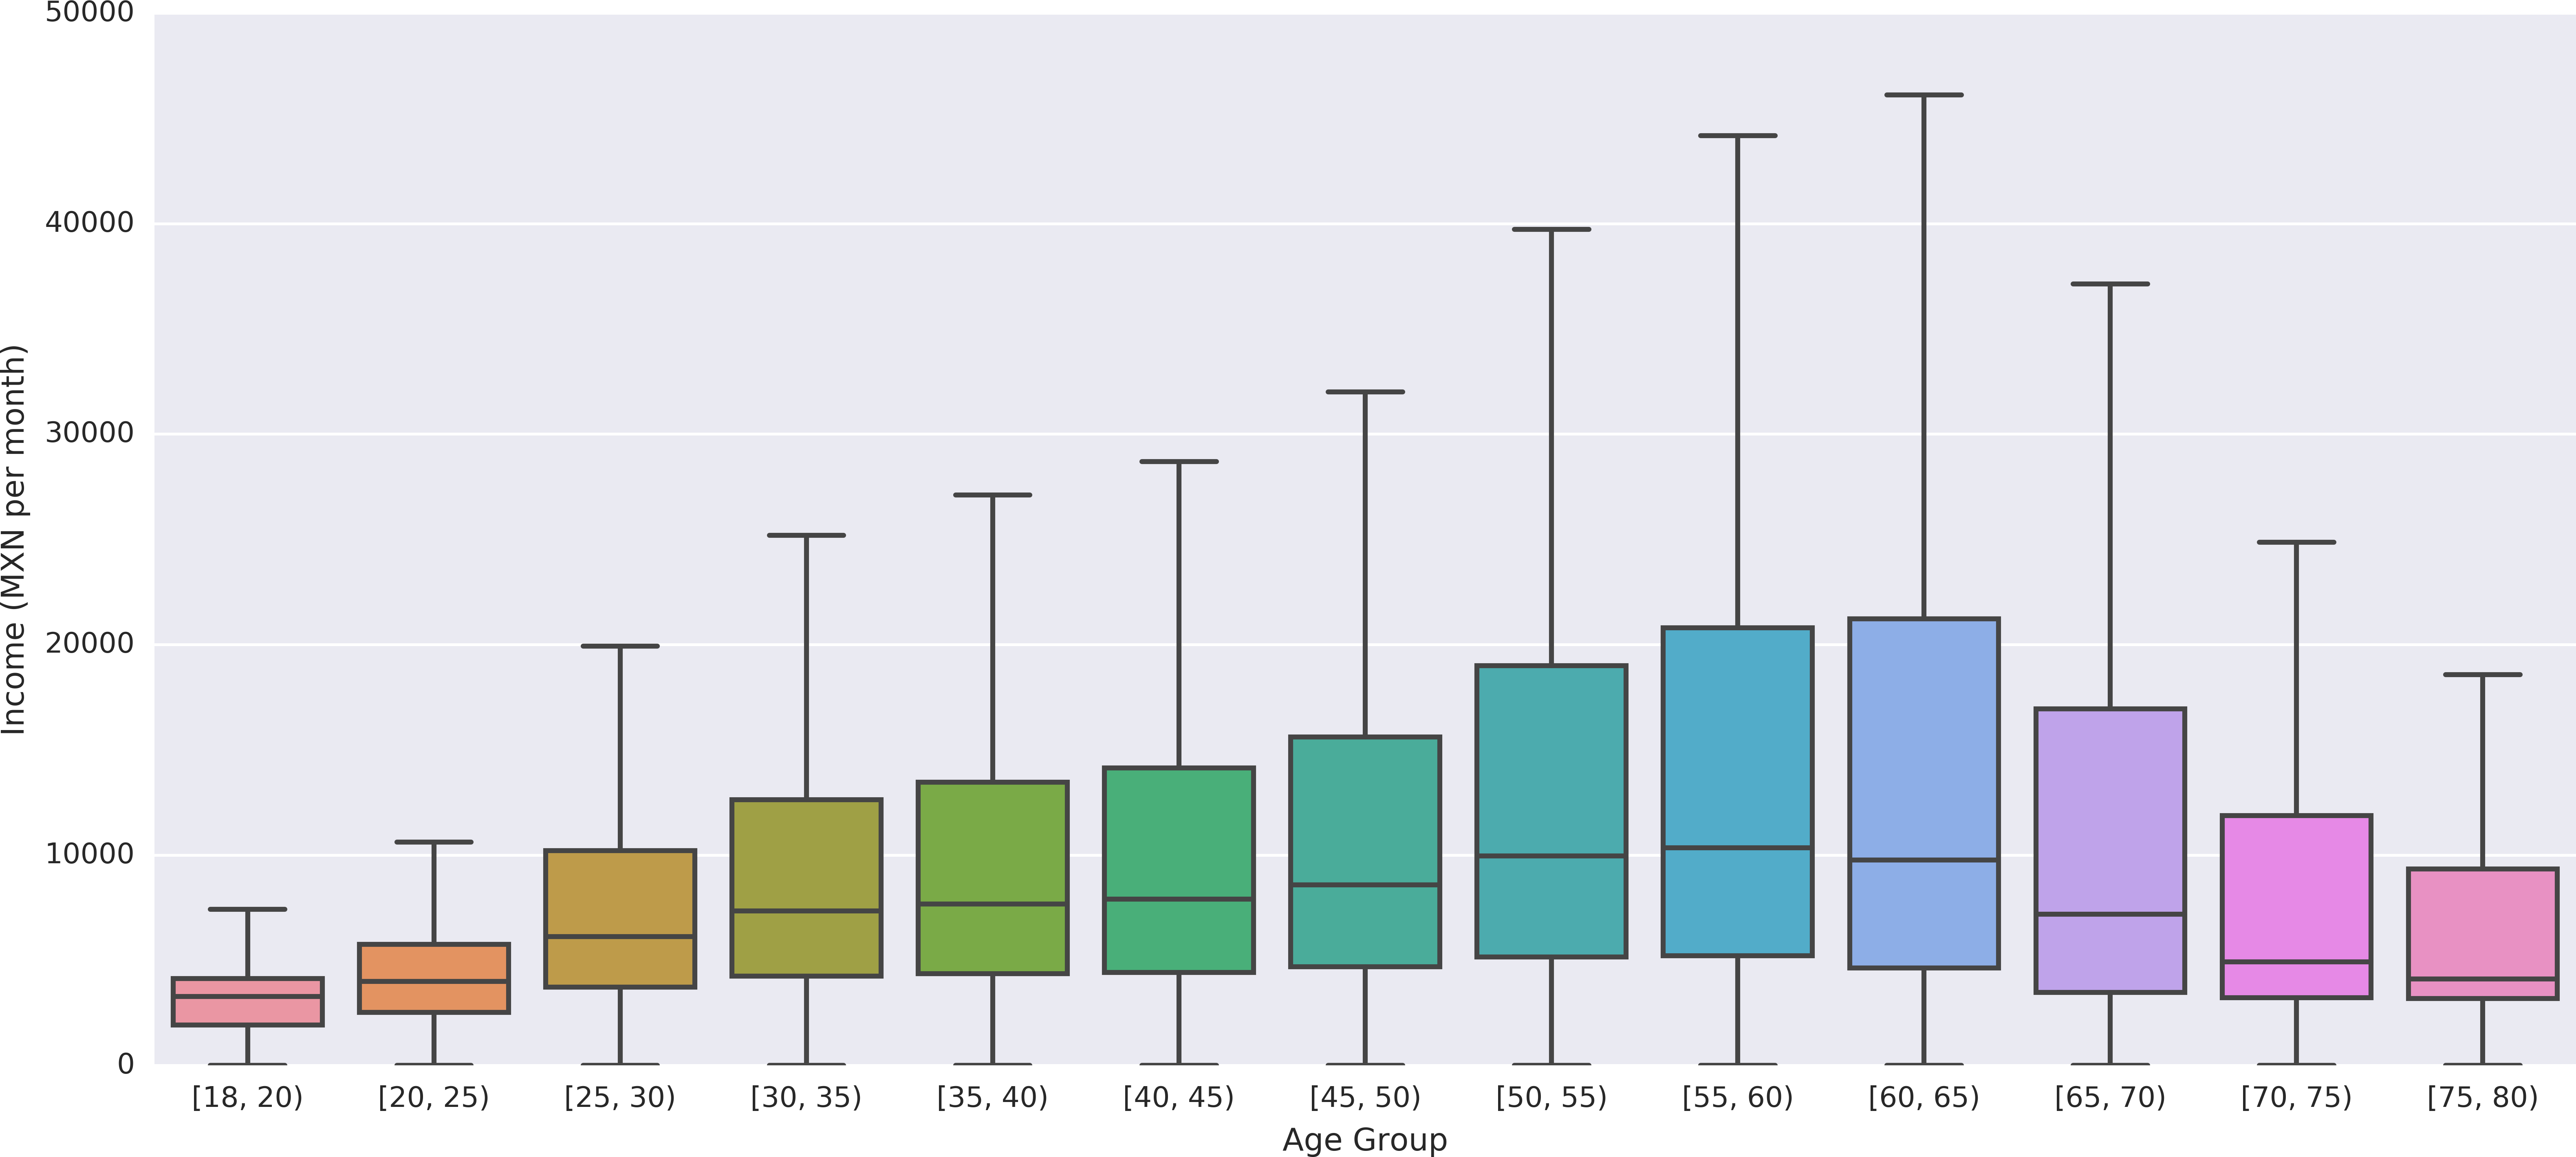
\includegraphics[width=\columnwidth]
				{../figures/income_age_boxplot4/income_age_boxplot4_wide.png}
		}\label{income_age_boxplot}
	\end{center}
\end{figure}
\end{frame}

\subsection{Mobile Phone Data Source}

\begin{frame}{Mobile Phone Data Source}
The main dataset for this study consists of a set \( \mathP \) of \textit{Call Detail Records} composed of voice calls and text messages from a Mexican telco for a 3 month period. Since we only have complete data for users of the telco, we work on set of calls \( \mathG_N \) between these users.

\medskip

The data in \( \mathB \) contains the self-reported phone numbers of the bank user, which the bank hashes with the same function as the telco uses for the CDRs. Thanks to this fact, we can correlate telco users with bank users to create the \textbf{social graph} \( G \).
\[
	G = \mathP \bowtie_{\operatorname{originUser}} \mathB \bowtie_{\operatorname{targetUser}} \mathB
\]

This graph has a total of \num{2027554} nodes with \num{5044976} edges, which represent \num{29599762} calls and \num{5476783} text messages.
\end{frame}

\section{Inference Methodology}
\subsection{Income Homophily}

\begin{frame}{Inference Methodology}
The main part of this work is based on the observed homophily between income levels of the participants in a phone call. That is, if person \emph{X} calls person \emph{Y}, then there's a high change that \emph{X} and \emph{Y} have similar incomes.
	
We can observe this homophily in the source data by measuting \textbf{Spearman's Rank Correlation} to test the statistical dependence of sets \emph{X} and \emph{Y}.

\[
	r_s = \mathlarger{\rho}_{\operatorname{rank}(X) \operatorname{rank}(Y)} = \frac{\operatorname{cov}(\operatorname{rank}(x), \operatorname{rank}(y))}{\sigma_{\operatorname{rank}(X)} \sigma_{\operatorname{rank}(Y)}}
\]

This formula gives us a correlation coefficient of \( \mathbf{r_s = 0.474} \). Compared to a randomized null hypothesis, where links between users are selected randomly disregarding income data, we have a p-value of \( p < 10^{-6} \).

\end{frame}
\begin{frame}

\begin{figure}[h]
	\begin{center}
		{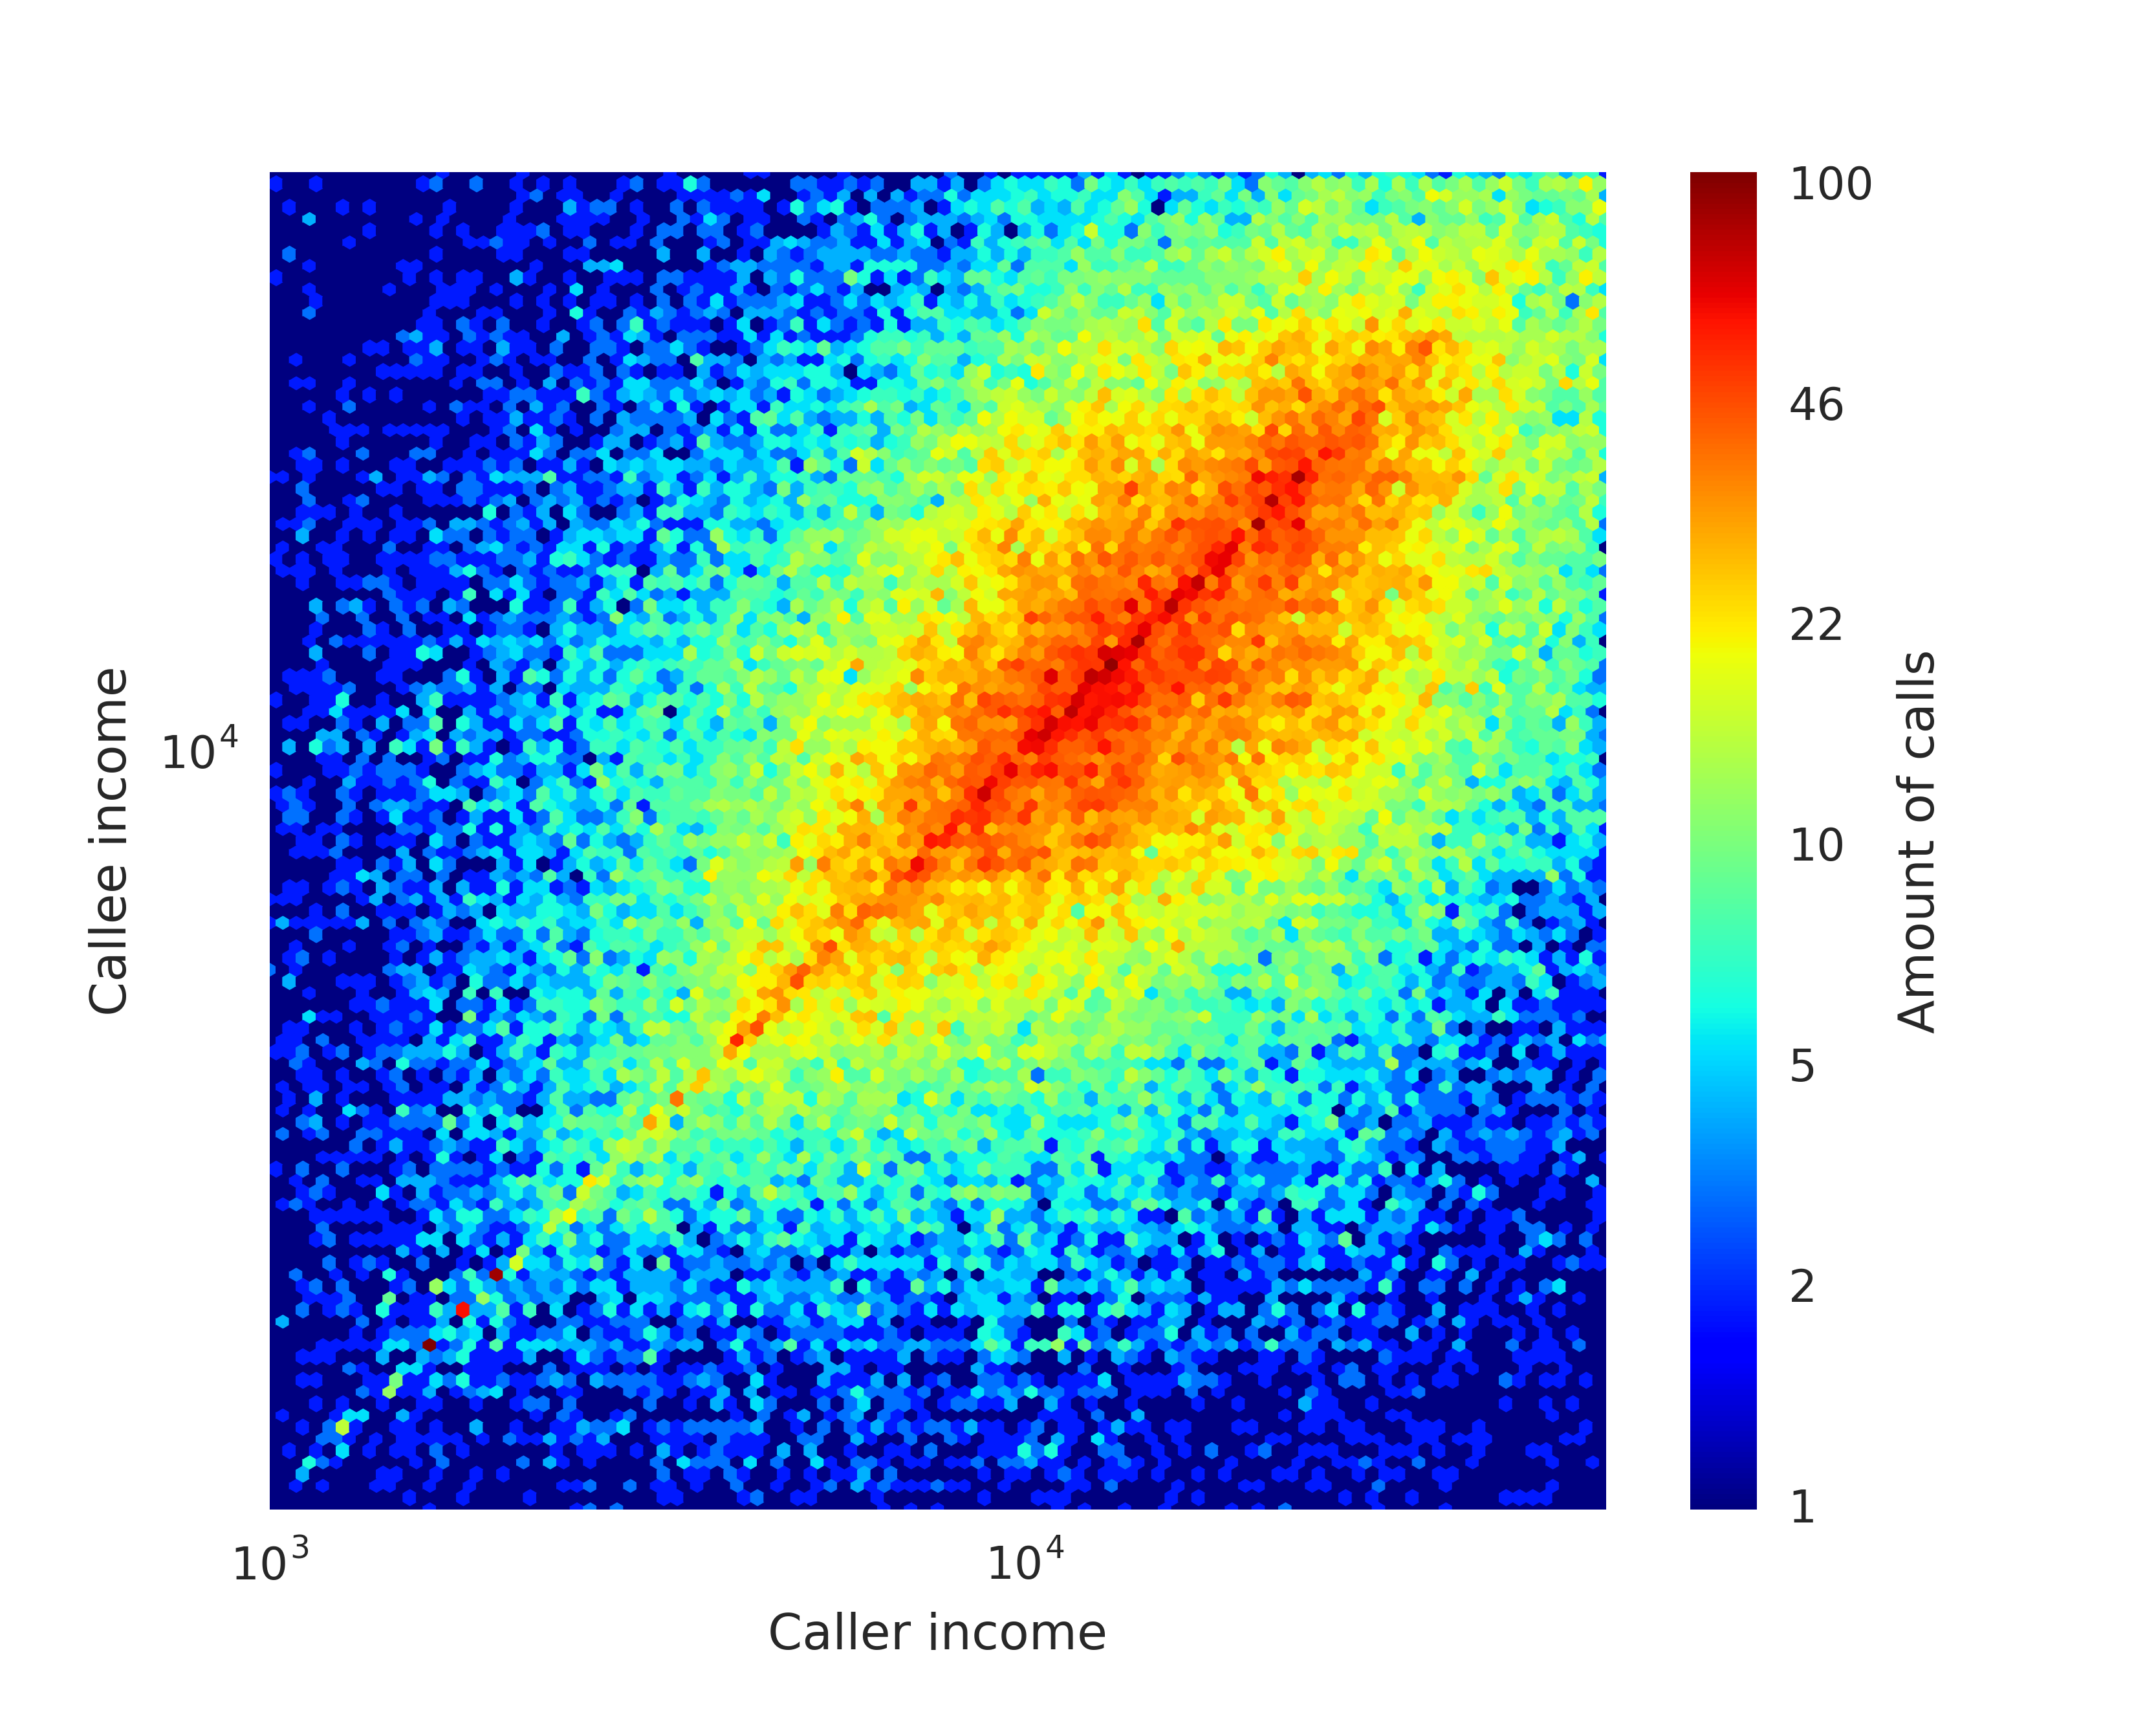
\includegraphics[height=0.8\textheight]
		{../figures/Homophily_income_origin_target_1/Homophily_income_origin_target_1.png}
		}\label{homophily_heatmap}
	\end{center}
	\caption{The income homophily can be easily seen when plotting the data.}
\end{figure}

\end{frame}

\subsection{Prediction Algorithm}
\begin{frame}{Prediction Algorithm}
	We separate the users in our input into two disjoint groups:

	\begin{description}
		\item[Poor People] have less than 3600~MXN\footnote{3600~MXN = 343~USD = 5095ARS} in their bank account.
		\item[Wealthy People] have more than 3600~MXN.\@
	\end{description}

	According to our hypothesis, poorer people should have more calls to other poor people, while wealthy people should have more calls to wealthier ones.

\end{frame}

\end{document}
